\documentclass[a4paper]{article}

\usepackage[utf8]{inputenc}
\usepackage[T1]{fontenc}
\usepackage{textcomp}
\usepackage{amsmath, amssymb}
\usepackage{amsthm}
\usepackage{physics}
\usepackage{subfig}
\usepackage{graphicx}
\usepackage[outdir=./]{epstopdf}

\DeclareMathOperator{\R}{\mathbb{R}}
\DeclareMathOperator{\C}{\mathbb{C}}
\DeclareMathOperator{\N}{\mathbb{N}}
\DeclareMathOperator{\Z}{\mathbb{Z}}

\title{Revision}
\author{Ernesto Camacho Ramírez}
\begin{document}
  \maketitle

  \section{DPS Graphs}

  \begin{figure}[ht]%
    \centering
    \subfloat[\centering $\phi = 0$ (ray bundle)
	]{{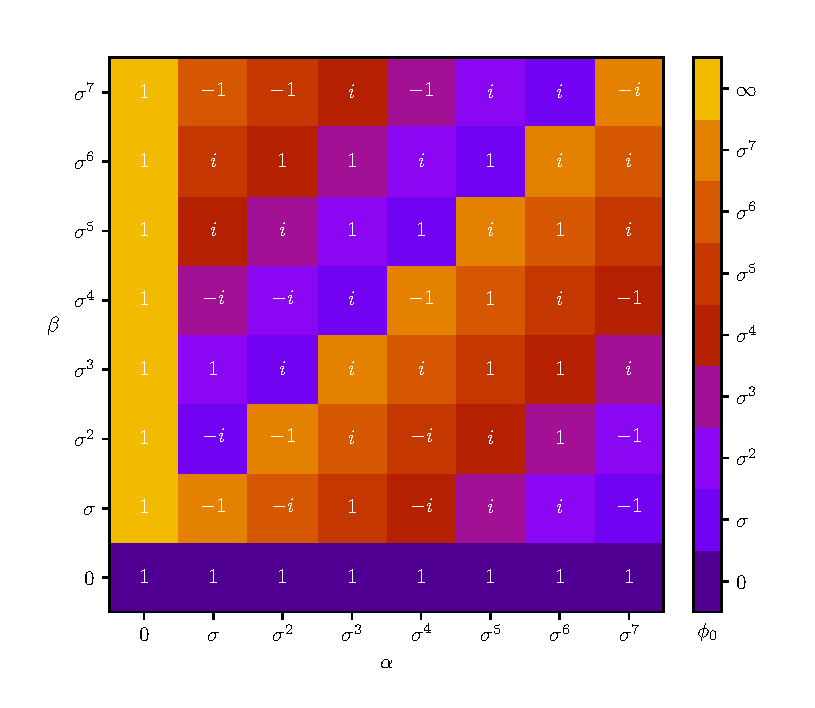
\includegraphics[width=0.5\textwidth]{DPS_rays_heat.eps} }}%
	%\quad
    \subfloat[\centering $\phi = 1$ (a $(1,6,2)$ bundle)
	]{{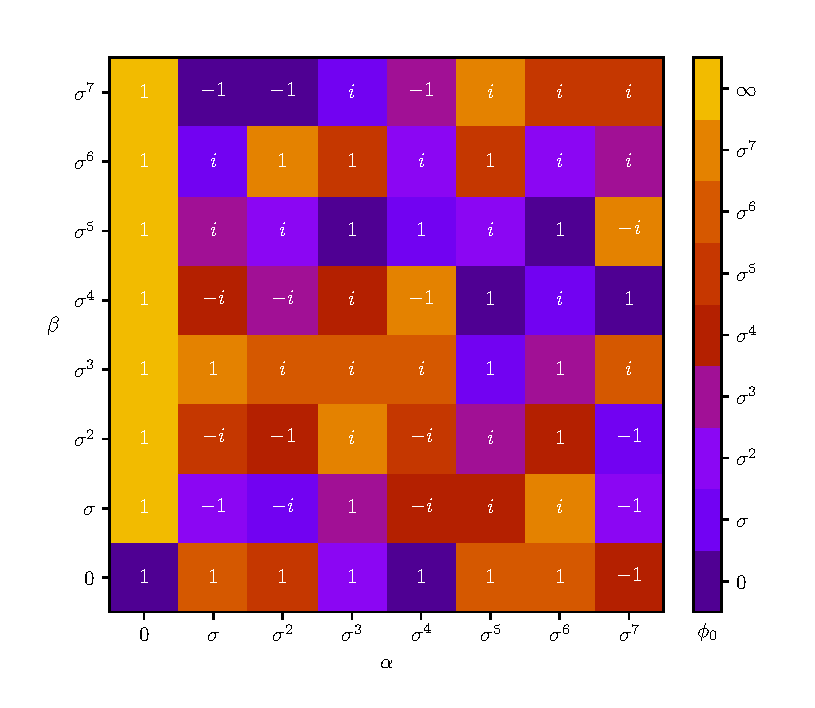
\includegraphics[width=0.5\textwidth]{DPS_curve_heat.eps} }}%
	\caption{
      Here we show the discrete phase space for two
      different bundles of regular curves whose general form
      is $\beta = \phi_0 \alpha + \phi^2 \alpha^2 + \phi
      \alpha^{4}$, where $\phi_0 \in \mathbb F_{2^3}$. At
      each point we assign the corresponding phase
      calculated by Eq. (\ref{Phi G}) choosing the all
      positive basis solution. The first DPS corresponds to
      $\phi = 0$, which gives us the rays; while the second
      DPS corresponds to $\phi = 1$, which gives us a bundle
      with factorization $(1,6,2)$.
	}%
    \label{fig-DPS}%
  \end{figure}

  
  \section{State Tomography Example}

  We can express the projection operator onto the
  $\kappa$-th eigenstate assigned to the striation of curves
  $\Gamma^\lambda$ as a sum of displacement operators:
  \begin{equation}
    \ket{\psi_\kappa^{\lambda}}
    \bra{\psi_\kappa^{\lambda}}
    = \frac{1}{2^{N}} \sum_{\tau}^{} 
    \chi(\kappa \tau) D(\alpha(\tau), \beta(\tau)),
  \end{equation}
  For example, the eigenstate assigned to the $\kappa = 0$
  curve of the striation that contains the abelian curve
  $\lambda$ given by Ec. (\ref{ac2}), $\beta = \alpha +
  \sigma^3 \alpha^2 + \sigma^{5} \alpha^{4}$, can be
  expressed as:
  \begin{equation}
    \ket{\psi_0^{\lambda}}
    \bra{\psi_0^{\lambda}}
    =
    \displaystyle \left(\begin{array}{rrrrrrrr}
    \frac{1}{4} & 0 & \frac{i}{4} & 0 & 0 & 0 & \frac{i}{4}
                & -\frac{1}{4} \\ [6pt]
    0 & 0 & 0 & 0 & 0 & 0 & 0 & 0 \\ [6pt]
    -\frac{i}{4} & 0 & \frac{1}{4} & 0 & 0 & 0 & \frac{1}{4}
                 & \frac{i}{4} \\ [6pt]
    0 & 0 & 0 & 0 & 0 & 0 & 0 & 0 \\ [6pt]
    0 & 0 & 0 & 0 & 0 & 0 & 0 & 0 \\ [6pt]
    0 & 0 & 0 & 0 & 0 & 0 & 0 & 0 \\ [6pt]
    -\frac{i}{4} & 0 & \frac{1}{4} & 0 & 0 & 0 & \frac{1}{4}
                 & \frac{i}{4} \\ [6pt]
    -\frac{1}{4} & 0 & -\frac{i}{4} & 0 & 0 & 0 &
    -\frac{i}{4} & \frac{1}{4}
    \end{array}\right)
  \end{equation}
  Similarly, using the appropriate phases, we can obtain the
  $\kappa = 0$ eigenstate of the striation given by the
  non-abelian curve $\lambda'$ with equation Ec. (\ref{nac})
  $\beta = \sigma^2 \alpha + \sigma^3 \alpha^2 + \sigma^{5}
  \alpha^{4}$:
  \begin{equation}
    \ket{\psi_0^{\lambda'}}
    \bra{\psi_0^{\lambda'}}
    =
    \displaystyle \left(\begin{array}{rrrrrrrr}
    \frac{1}{2} & \frac{i}{2} & 0 & 0 & 0 & 0 & 0 & 0 \\
    [6pt]
    -\frac{i}{2} & \frac{1}{2} & 0 & 0 & 0 & 0 & 0 & 0 \\
    [6pt]
    0 & 0 & 0 & 0 & 0 & 0 & 0 & 0 \\ [6pt]
    0 & 0 & 0 & 0 & 0 & 0 & 0 & 0 \\ [6pt]
    0 & 0 & 0 & 0 & 0 & 0 & 0 & 0 \\ [6pt]
    0 & 0 & 0 & 0 & 0 & 0 & 0 & 0 \\ [6pt]
    0 & 0 & 0 & 0 & 0 & 0 & 0 & 0 \\ [6pt]
    0 & 0 & 0 & 0 & 0 & 0 & 0 & 0
    \end{array}\right)
  \end{equation}
  We can use the complete set of MUBs used to create the
  Wigner kernel to reconstruct a state given the measured
  probabilities $p_{\kappa}^{\lambda} =
  \bra{\psi_\kappa^\lambda}\hat\rho\ket{\psi_\kappa^\lambda}$.
  The state can then be expressed as a sum of these
  projection operators as in Eq. (\ref{tom r}). This is a
  process called \textit{quantum state tomography}. For both
  states $\ket{\psi_0^{\lambda}}\bra{\psi_0^{\lambda}}$ and
  $\ket{\psi_0^{\lambda'}}\bra{\psi_0^{\lambda'}}$, we
  obtain four possible values for the measured probabilities
  using the MUBs of the ray bundle. These values are
  \begin{equation}
    p_\kappa^\mu
    \in 
    \left\{
      0, \frac{1}{8}, \frac{1}{4}, \frac{1}{2}
    \right\},
  \end{equation}
  where $\mu \in \mathbb F_{2^3}$ denotes the slope of the
  ray.
   

%La función de Wigner del estado correspondiente a la
  %curva abeliana es:
  %\begin{equation}
  %  W_\rho =
  %  \displaystyle \left(\begin{array}{rrrrrrrr}
  %  \frac{1}{8} & 0 & 0 & 0 & 0 & 0 & 0 & 0 \\ [6pt]
  %  0 & 0 & 0 & 0 & 0 & 0 & 0 & \frac{1}{8} \\ [6pt]
  %  \frac{1}{8} & 0 & 0 & 0 & 0 & 0 & 0 & 0 \\ [6pt]
  %  0 & 0 & \frac{1}{8} & 0 & 0 & 0 & 0 & 0 \\ [6pt]
  %  0 & 0 & 0 & 0 & 0 & 0 & 0 & \frac{1}{8} \\ [6pt]
  %  0 & 0 & \frac{1}{8} & 0 & 0 & 0 & 0 & 0 \\ [6pt]
  %  0 & 0 & 0 & 0 & 0 & 0 & \frac{1}{8} & 0 \\ [6pt]
  %  0 & 0 & 0 & 0 & 0 & 0 & \frac{1}{8} & 0
  %  \end{array}\right)
  %\end{equation}

  \section{Phases for two qutrits}

  Let $\mathbb F_{3^2}$ be the finite field of nine elements
  with irreducible polynomial $x^2 + 2x + 2$. We use the
  almost self-dual basis $\{1, \sigma^2\}$ for all
  calculations. Since we are dealing with odd local
  dimension, the phase $\Phi_{\alpha,\beta}(\tau)$ is unique
  and is given by Eq. (\ref{Phio}). This implies that all
  discrete phase space structures will have the same phases
  and in our case it is given by:
  \begin{equation}
    \Phi =
    \displaystyle \left(\begin{array}{rrrrrrrrrr}
    \alpha \backslash \beta & 0 & \sigma & \sigma^2 &
    \sigma^3 & \sigma^4 & \sigma^5 & \sigma^6 & \sigma^7 & \sigma^8 \\
    0 & 1 & 1 & 1 & 1 & 1 & 1 & 1 & 1 & 1 \\
    \sigma & 1 & 1 & \omega & \omega & \omega^{2} & 1 & \omega^{2} & \omega^{2} & \omega \\
    \sigma^2 & 1 & \omega & \omega & \omega^{2} & 1 & \omega^{2} & \omega^{2} & \omega & 1 \\
    \sigma^3 & 1 & \omega & \omega^{2} & 1 & \omega^{2} & \omega^{2} & \omega & 1 & \omega \\
    \sigma^4 & 1 & \omega^{2} & 1 & \omega^{2} & \omega^{2} & \omega & 1 & \omega & \omega \\
    \sigma^5 & 1 & 1 & \omega^{2} & \omega^{2} & \omega & 1 & \omega & \omega & \omega^{2} \\
    \sigma^6 & 1 & \omega^{2} & \omega^{2} & \omega & 1 & \omega & \omega & \omega^{2} & 1 \\
    \sigma^7 & 1 & \omega^{2} & \omega & 1 & \omega & \omega & \omega^{2} & 1 & \omega^{2} \\
    \sigma^8 & 1 & \omega & 1 & \omega & \omega & \omega^{2} & 1 & \omega^{2} & \omega^{2}
    \end{array}\right),
  \end{equation}
  where $\omega = e^{2\pi i / 3}$. 

  %We can create the partition of the DPS using a bundle of
  %curves just as in the qubit case. The difference is that
  %the phases won't change depending on the bundle chosen for
  %the partition. The following figure shows the DPS for the
  %rays.

  Since the phase $\Phi(\alpha,\beta) =
  \chi(-2^{-1}\alpha\beta) = \chi(\alpha\beta)$ factors as
  the product
  \begin{equation}
    \prod_i^n \omega^{\alpha_i \beta_i q_i},
  \end{equation}
  we can express the phase space $\Phi$ above as an element
  wise product of matrices:
  \begin{align}
    & \left(\begin{array}{rrrrrrrrr}
      1 & 1 & 1 & 1 & 1 & 1 & 1 & 1 & 1 \\
      1 & 1 & \omega & \omega & \omega^{2} & 1 & \omega^{2} & \omega^{2} & \omega \\
      1 & \omega & \omega & \omega^{2} & 1 & \omega^{2} & \omega^{2} & \omega & 1 \\
      1 & \omega & \omega^{2} & 1 & \omega^{2} & \omega^{2} & \omega & 1 & \omega \\
      1 & \omega^{2} & 1 & \omega^{2} & \omega^{2} & \omega & 1 & \omega & \omega \\
      1 & 1 & \omega^{2} & \omega^{2} & \omega & 1 & \omega & \omega & \omega^{2} \\
      1 & \omega^{2} & \omega^{2} & \omega & 1 & \omega & \omega & \omega^{2} & 1 \\
      1 & \omega^{2} & \omega & 1 & \omega & \omega & \omega^{2} & 1 & \omega^{2} \\
      1 & \omega & 1 & \omega & \omega & \omega^{2} & 1 & \omega^{2} & \omega^{2}
      \end{array}\right) \\
    &= \underbrace{
    \left(\begin{array}{rrrrrrrrr}
    1 & 1 & 1 & 1 & 1 & 1 & 1 & 1 & 1 \\
    1 & \omega^{2} & 1 & \omega^{2} & \omega^{2} & \omega & 1 & \omega & \omega \\
    1 & 1 & 1 & 1 & 1 & 1 & 1 & 1 & 1 \\
    1 & \omega^{2} & 1 & \omega^{2} & \omega^{2} & \omega & 1 & \omega & \omega \\
    1 & \omega^{2} & 1 & \omega^{2} & \omega^{2} & \omega & 1 & \omega & \omega \\
    1 & \omega & 1 & \omega & \omega & \omega^{2} & 1 & \omega^{2} & \omega^{2} \\
    1 & 1 & 1 & 1 & 1 & 1 & 1 & 1 & 1 \\
    1 & \omega & 1 & \omega & \omega & \omega^{2} & 1 & \omega^{2} & \omega^{2} \\
    1 & \omega & 1 & \omega & \omega & \omega^{2} & 1 & \omega^{2} & \omega^{2}
    \end{array}\right)
    }_{
      \omega^{\alpha_1  \beta_1 q_1},
      \; \alpha_1 = \tr(\alpha\theta_1),
      \; \beta_1 = \tr(\beta\theta_1)
    }
    \odot
    \underbrace{
      \left(\begin{array}{rrrrrrrrr}
      1 & 1 & 1 & 1 & 1 & 1 & 1 & 1 & 1 \\
      1 & \omega & \omega & \omega^{2} & 1 & \omega^{2} & \omega^{2} & \omega & 1 \\
      1 & \omega & \omega & \omega^{2} & 1 & \omega^{2} & \omega^{2} & \omega & 1 \\
      1 & \omega^{2} & \omega^{2} & \omega & 1 & \omega & \omega & \omega^{2} & 1 \\
      1 & 1 & 1 & 1 & 1 & 1 & 1 & 1 & 1 \\
      1 & \omega^{2} & \omega^{2} & \omega & 1 & \omega & \omega & \omega^{2} & 1 \\
      1 & \omega^{2} & \omega^{2} & \omega & 1 & \omega & \omega & \omega^{2} & 1 \\
      1 & \omega & \omega & \omega^{2} & 1 & \omega^{2} & \omega^{2} & \omega & 1 \\
      1 & 1 & 1 & 1 & 1 & 1 & 1 & 1 & 1
      \end{array}\right)
    }_{
      \omega^{\alpha_2 \beta_2 q_2},
      \; \alpha_2 = \tr(\alpha\theta_2),
      \; \beta_2 = \tr(\beta\theta_2)
    }
  \end{align}
  
\end{document}
